\subsubsection{Network Topology Before and After Market-Mode Removal}
\label{sec:networks}

The hierarchical analysis showed that localized dependency patterns remain after removal of the dominant market component, although the resulting geometry becomes less purely tree-like. We therefore move to graph-based representations, which retain selected dependency links and allow changes in connectivity, local organization, and centrality to be examined directly. We compare networks constructed from the original correlation matrix with those obtained from the group-mode component identified through RMT.

The Minimum Spanning Tree (MST) provides the sparsest connected representation of the dependency structure. With $N=58$ assets, each MST contains 57 edges. Figure~\ref{fig:mst_refined} compares the original and group-mode backbones.

\begin{center}
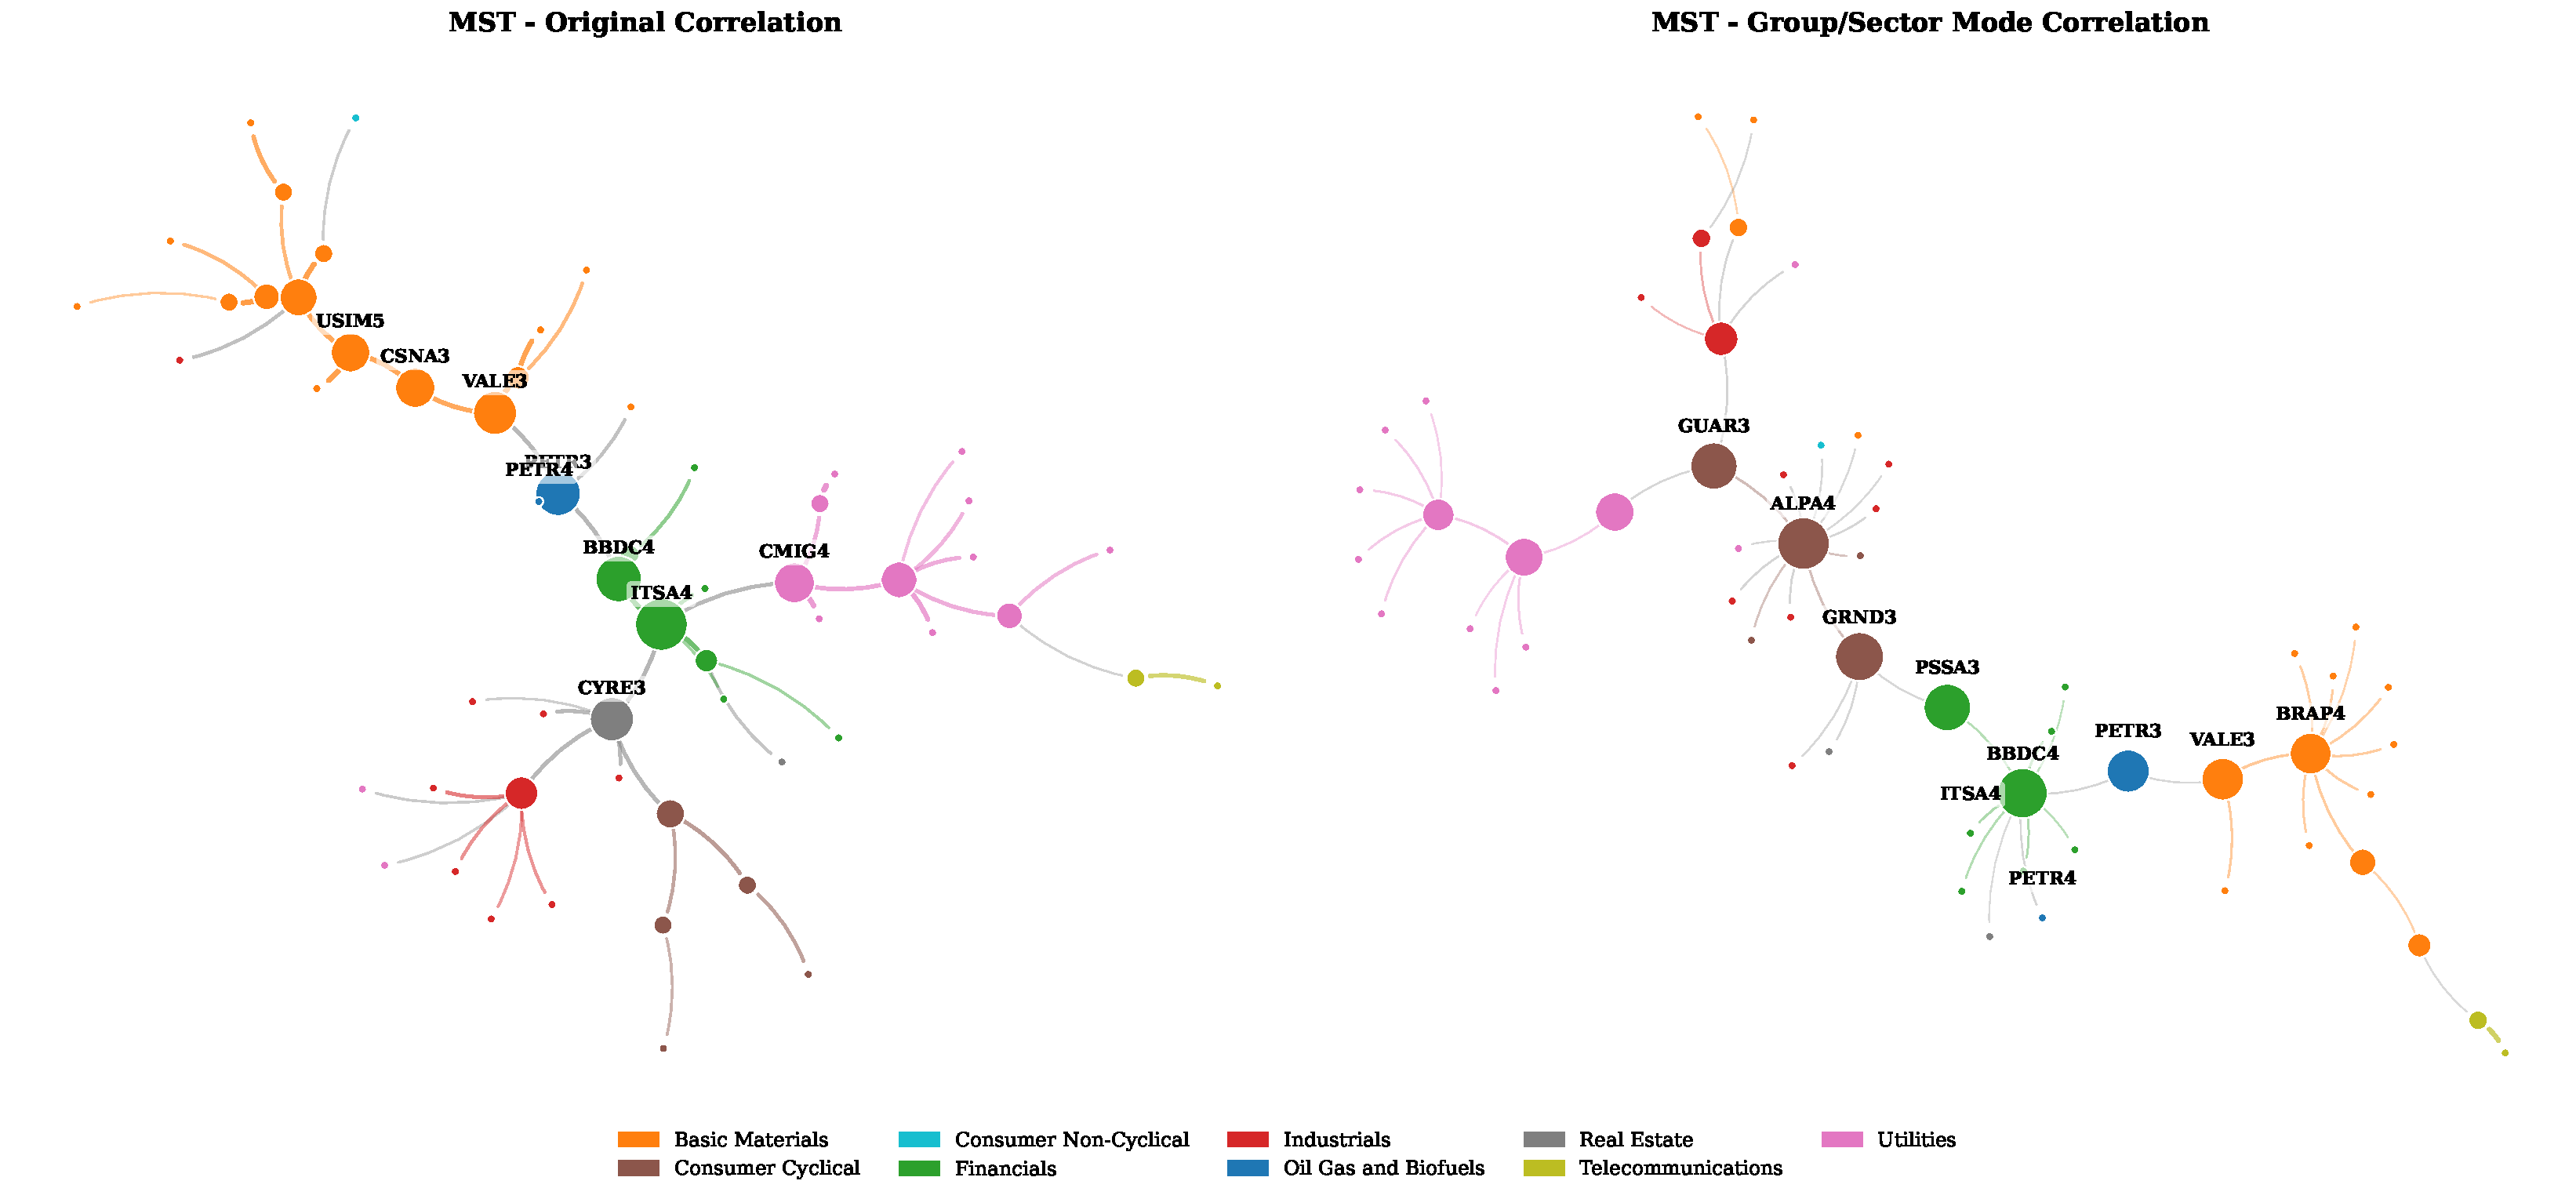
\includegraphics[
width=\linewidth,
height=0.58\textheight,
keepaspectratio
]{images/figure_11b_mst_refined_comparison.pdf}
\captionof{figure}{MST comparison for the original and group-mode correlation structures. Removal of the dominant market component changes the set of strongest dependency channels retained in the network backbone.}
\label{fig:mst_refined}
\end{center}

The original MST has a mean edge correlation of 0.5796, compared with 0.1388 for the group-mode MST. This reduction is expected because the latter excludes the dominant common component. More importantly, the same-sector edge ratio decreases from 0.7193 to 0.6316, indicating that the topology is reorganized rather than simply weakened. The group-mode MST therefore represents a different dependency backbone, emphasizing relationships that remain after broad market synchronization is removed.

The Planar Maximally Filtered Graph (PMFG) provides a richer representation of the same dependency geometry. Unlike the MST, the PMFG retains $3N-6=168$ edges and allows cycles, triangles, and cliques to remain in the graph. Figure~\ref{fig:pmfg_refined} compares the original and group-mode PMFGs.

\begin{center}
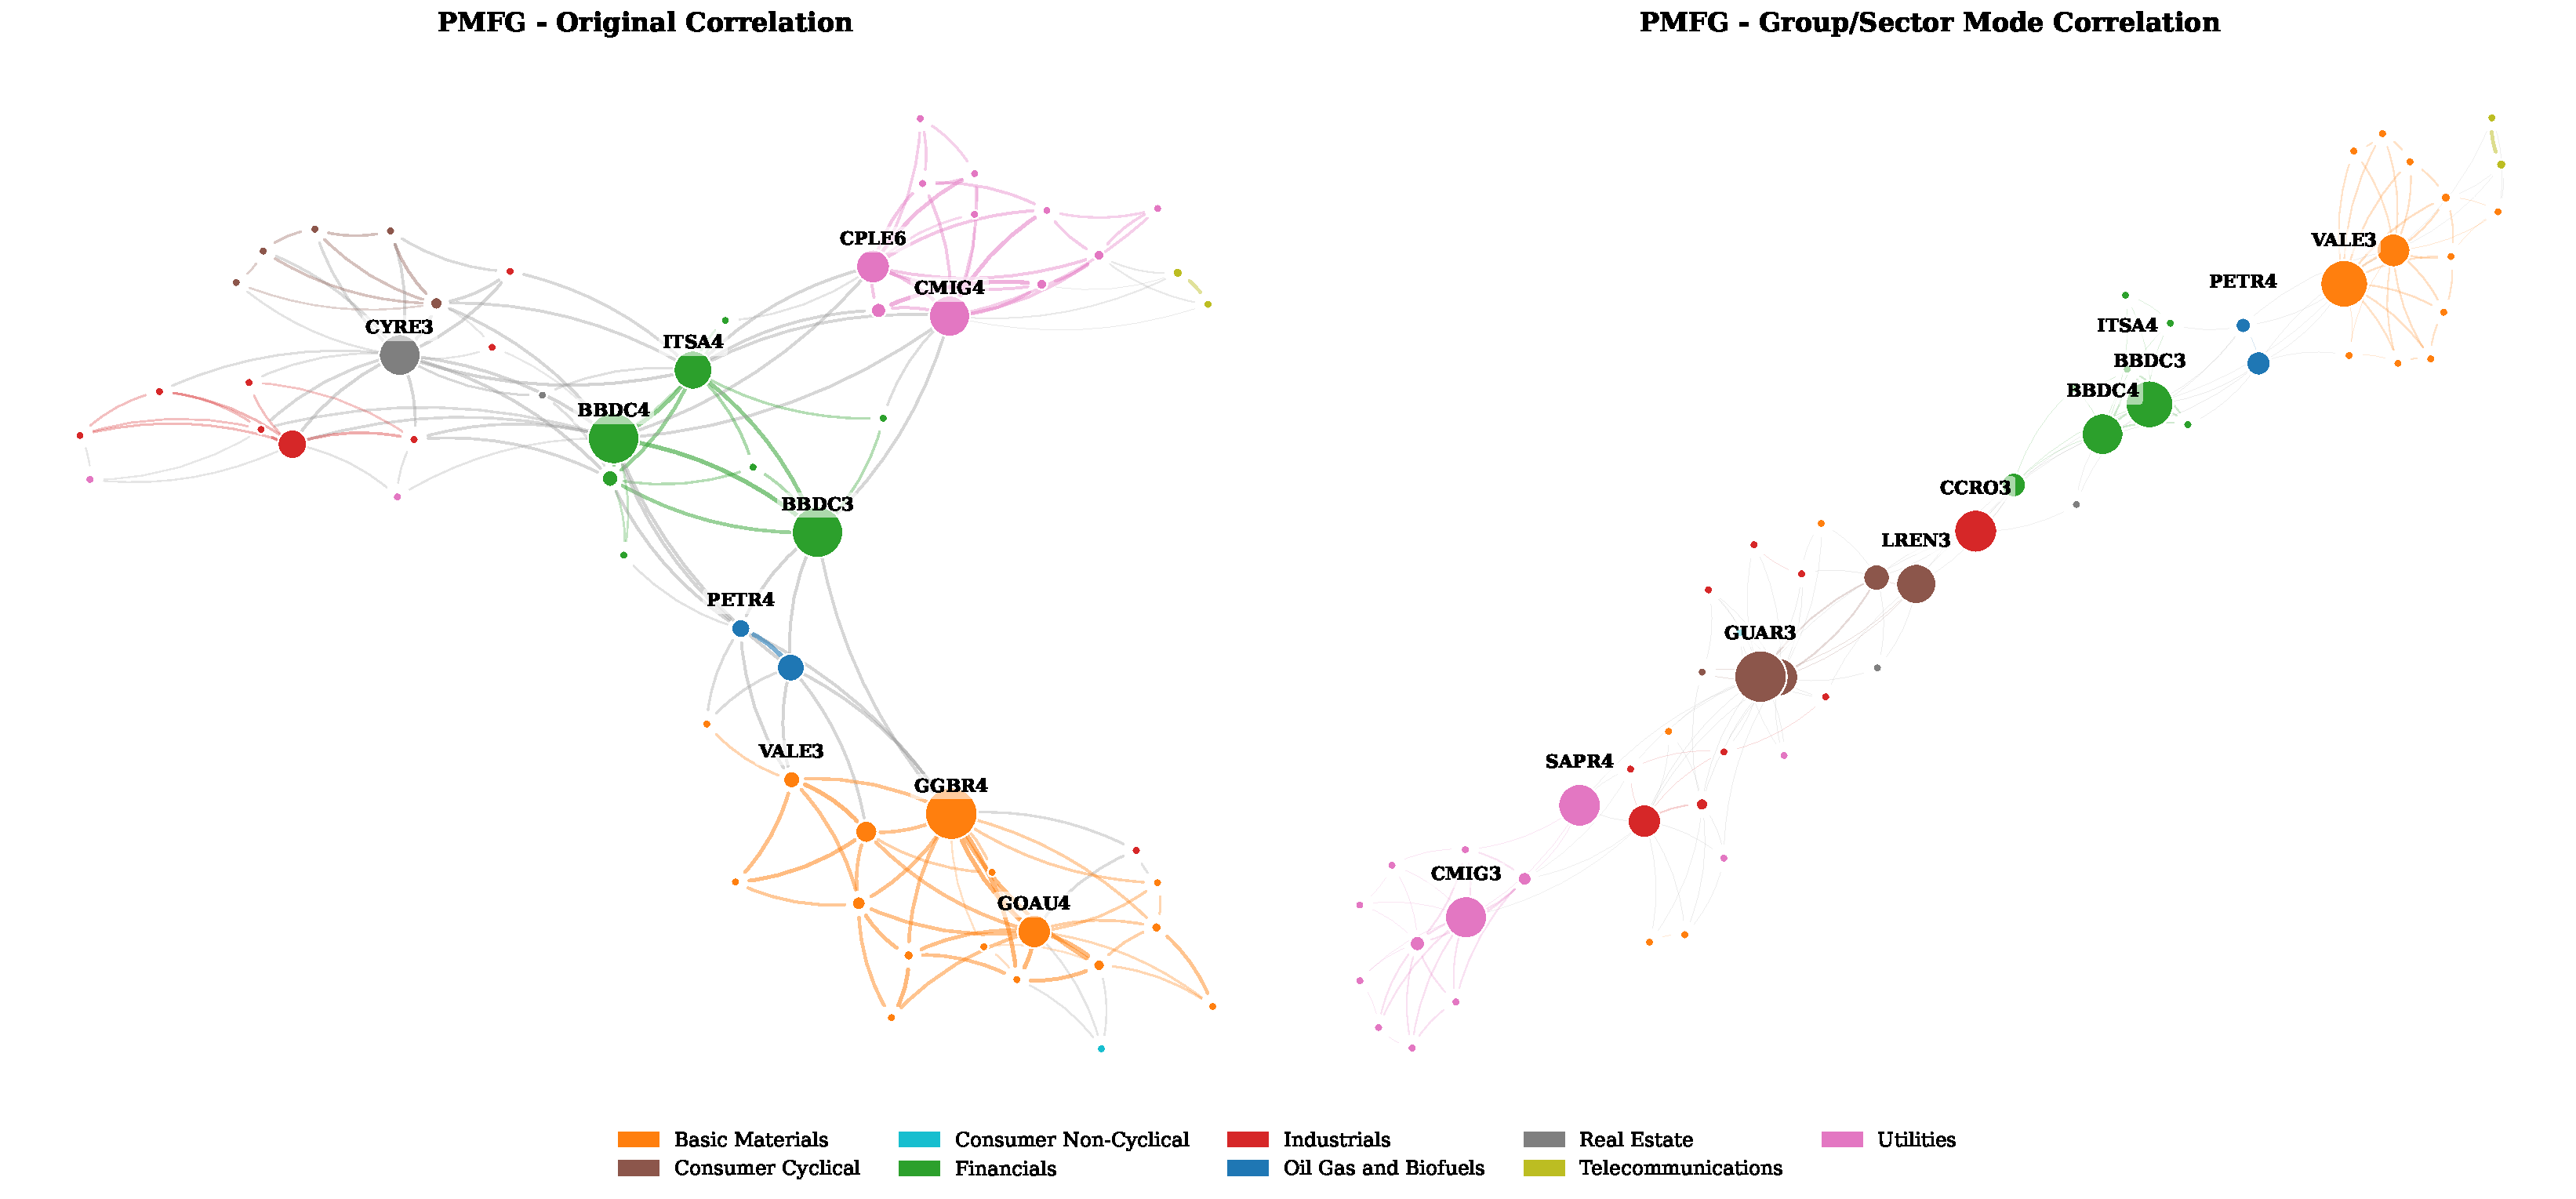
\includegraphics[
width=\linewidth,
height=0.58\textheight,
keepaspectratio
]{images/figure_12b_pmfg_refined_comparison.pdf}
\captionof{figure}{PMFG comparison for the original and group-mode correlation structures. The group-mode representation removes broad market-wide dominance while retaining a denser set of localized dependency relationships.}
\label{fig:pmfg_refined}
\end{center}

As in the MST, average edge strength decreases substantially after market-mode removal, from 0.5177 in the original PMFG to 0.1109 in the group-mode PMFG. The topological response, however, is not a uniform loss of structure. Average clustering increases from 0.5273 to 0.6653, while the same-sector edge ratio decreases from 0.6012 to 0.5417. Thus, weaker absolute correlations coexist with stronger local triangular organization after removal of the broad market component.

Table~\ref{tab:network_summary} summarizes the main differences across the two graph families.

\begin{center}
\captionof{table}{Selected topology statistics for the original and group-mode MST and PMFG representations.}
\label{tab:network_summary}
\small
\setlength{\tabcolsep}{3.5pt}
\begin{tabular}{llrrrrrr}
\toprule
Network & Matrix & Edges & Mean corr. & Same-sector & Clustering & Top degree & Top betweenness \\
\midrule
MST & Original & 57 & 0.5796 & 0.7193 & 0.0000 & RAPT4 & ITSA4 \\
MST & Group mode & 57 & 0.1388 & 0.6316 & 0.0000 & ALPA4 & ALPA4 \\
PMFG & Original & 168 & 0.5177 & 0.6012 & 0.5273 & BBDC4 & GGBR4 \\
PMFG & Group mode & 168 & 0.1109 & 0.5417 & 0.6653 & GUAR3 & GUAR3 \\
\bottomrule
\end{tabular}
\end{center}


The comparison reveals a consistent pattern across MST and PMFG representations. Removing the dominant market mode substantially reduces edge strength and partially reduces sectoral concentration, but it does not eliminate organized dependency structure. In the PMFG, the simultaneous reduction in average correlation and increase in clustering is particularly informative: the residual network is weaker in absolute correlation terms but more locally organized around interconnected groups of assets.

The PMFG construction also retains the expected planar structure, with 168 edges, 166 triangles, and 55 four-cliques for the 58-asset network. These quantities are primarily construction diagnostics and are therefore reported in detail in the supplementary material. Their main role here is to confirm that the PMFG preserves local structures that cannot appear in the MST. The remaining question is whether removal of the market mode also changes which assets occupy structurally important positions. We therefore examine hub reorganization next.
